\todo{Make sure that all $k$-space functions have tildes.  Or not, but be
consisitent with other chapters.}
When surface plasmon polaritons are excited in a prism coupled setup using
a focused beam, a curious one-sided oscillation pattern appears in both the
reflected and scattered light~\cite{webster2013interference}.  For normal
SPPs observation of such typically requires the addition of an imaging
lens, but for LRSPPs it may be observed without one.  Surprisingly, despite
the ubiquity of SPR this phenomena went unreported until
2005~\cite{schumann2008near}~\cite{andaloro2005optical}, and have since
then only been reported in a handful of limited
cases~\cite{shan2009measuring}~\cite{simon2007observation}. 

\section{Existence}
For simplicity in our analysis we restrict the problem to the two
dimensional $x$-$z$ plane.  Consider an incident $p$-polarized Gaussian
beam passing through a prism exciting either normal or long range SPPs.  We
define this Gaussian beam $\tilde{g}(k_x)$ in $k$-space as an angular
spectrum of plane waves via Fourier decomposition
\begin{align}
\tilde{g}(k_x) &= \intinfty g(x)\, \me^{\mi k_x x} \md x\\
&=\me^{-k_x^2/w_0^2}
\end{align}
where $w_0$ denotes the Gaussian beam waist parameter at the focus.  In the
specular direction, the field $\tilde{E}_\mathrm{notch}(k_x)$ is given by its
Fresnel reflectivity multiplied by this Gaussian beam.
\begin{equation}
\tilde{E}_\mathrm{notch}(k_x)=\tilde{g}(k_x)\,\tilde{r}(k_x)
\end{equation}
where $\tilde{r}(k_x)$ is the Fresnel reflectivity for $p$-polarization.
In this chapter we will omit the superscript.

Let us now consider the spatial evolution of this function.  
The complete optical field in both $x$ and $z$ can be obtained by computing
the Fourier transform of $\tilde{E}_\mathrm{notch}(k_x)$ multiplied 
by the free space transfer function $\me^{\mi k_{z} z}$
\begin{align}
E_\mathrm{notch}(x,z) &= \intinfty \tilde{E}_\mathrm{notch}\, \me^{\mi k_{z,1} z}\, \me^{\mi k_x x} \md k_x\\
 &= \intinfty \tilde{g}(k_x)\, \tilde{r}(k_x)\, \me^{\mi \sqrt{k_0^2 \epsilon_1 - k_x^2}z}\, \me^{\mi k_x x} \md k_x
\label{eqn:fourier123}
\end{align}
Likewise, conically scattered light may be found using the same treatment
\begin{align}
E_\text{cone}(x,z) = \intinfty \tilde{g}(k_x)\, 
\tilde{t}_+(k_x)\, \tilde{t}_-(k_x)\,\me^{\mi k_z z}\, \me^{\mi k_x x} \md k_x
\label{eqn:fourier321}
\end{align}
Though this integral seems to have no analytic solution, its evaluation is
nonetheless straightforward on a computer.

\begin{figure}[ht]
 \centering
 \import{includes/}{setpgfinc}
	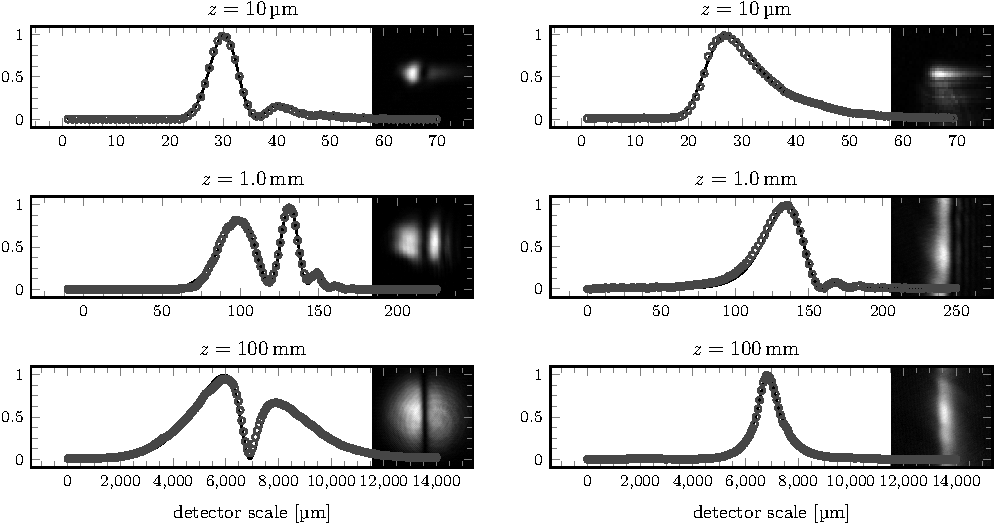
\includegraphics{interference/figures/fig2-crop.pdf}
 \caption{Fresnel Guys.}
 \label{fig:fresnelprop}
\end{figure}
The evolution of the notch and the cone based on
\Equation{eqn:fourier123} and \Equation{eqn:fourier321} is shown in
\Figure{fig:fresnelprop}.

\subsection{Evanescent Solutions}
In the context of diffraction integrals, the free space transfer function
$\exp(\mi k_{z,1} z)$ is often concerned with evanescent and propagating
terms, giving rise to the diffraction limit.  Here,
$k_{z,1}=\sqrt{k_0^2 \epsilon_1 - k_x^2}$ is imaginary for $k_0^2
\epsilon_1 < k_x^2$.  It is interesting to note that this never occurs.
Ignoring the condition for total internal reflection, 
$k_x = k_0 \sqrt{\epsilon_1} \sin \theta$ and we can set up an inequality
\begin{align}
k_0^2 \epsilon_1 &< k_x^2\\
k_0^2 \epsilon_1 &< \left(k_0 \sqrt{\epsilon_1} \sin \theta\right)^2\\
k_0^2 \epsilon_1 &< k_0^2 \epsilon_1 \sin^2 \theta\\
1 &< \sin^2 \theta
\end{align}
which is false, suggesting that if all light is collected, no information is
lost during propagation from the near to far field.
\section{The Fourier Optics Perspective}
There are several perspectives of SPR phenomena which can be insightful in
explaining why exactly the spatial oscillations are one-sided.  The first
is an argument from causality.  Assume a complex function $\chi(\omega) =
\chi'(\omega) + \mi \chi''(\omega)$ whose real and imaginary parts are
related by Kramers-Kronig relations
\begin{align}
\chi(\omega)=\mi \hf{\chi(\omega)}
\end{align}
with 
\begin{align}
\chi'(\omega) &= \hf{\chi''(\omega)}\\
\chi''(\omega) &= -\hf{\chi'(\omega)}
\end{align}
where $\hf{\chi(\omega)}$ is the Hilbert transform of $\chi(\omega)$.
The Fourier transform of $\chi(\omega)$ is
\begin{align}
\chi(\omega) &= \chi'(\omega) + \mi \chi''(\omega)\\
\ff{\chi(\omega)} &= \ff{\chi'(\omega) + \mi \chi''(\omega)}\\
&= \ff{\chi'(\omega)} + \ff{\mi \chi''(\omega)}\\
&= \ff{\chi'(\omega)} + \ff{\mi \hf{\chi'(\omega)}} \\
&= \ff{\chi'(\omega)} + \sgn(\omega) \ff{\chi'(\omega)} \\
\end{align}
Or succinctly,
\begin{align}
\ff{\hf{\chi(\omega)}} = (-\mi \sgn(\omega)) \ff{\chi(\omega)}
\end{align}
In other words, the Fourier transform of any function which satisfies
Kramers-Kronig relations is ``one-sided'' as a necessary
condition of causality.  This seems to be true for the Fresnel
reflectivity as well as the complex permittivity.

The second perspective is couched in Fourier optics.  Here, because
SPR occurs at the focus of a Gaussian beam, it can be seen as a sort of
spatial filter which modifies the local $k$-vectors to produce
the resulting far field optical pattern.  If the SPR resonance condition is
sharp, the Fourier integral (\Equation{eqn:fourier123}) is truncated and
the discontinuity acts as a low pass filter for light.  The one-sided
oscillations are then essentially a manifestation of Gibb's phenomena.
This seems to be well supported, because if the SPR resonance is broadened,
say in the case of a BK7-Au-\ce{H2O} system, the interference is greatly
attenuated.


